\chapter{Further thoughts on kinetic dominance}
\label{chap:kt}

This is a brief chapter whose content is based on discussions since the release of the material in Chapter~\ref{chap:kd} as the publication by~\cite{Handley+2014}.
To recap, the classical equations of motion for single field inflation are
governed by:
%
\begin{align}
  \dot{H} + H^2 
  &= - \frac{1}{3\m^2}\left( \dot{\phi}^2 - V(\phi)\right)
  \label{eqn:kt:raychaudhuri}
  \\
  0 &= \ddot{\phi} + 3H\dot\phi + V^\prime{\phi}
  \label{eqn:kt:kleingordon}
\end{align}
%
We have proved that if these equations are integrated backward in time
they always begin on a solution in which $\dot\phi^2\gg V(\phi)$
(independent of the potential). This is demonstrated in
Figure~\ref{fig:kt:w}. In this regime, the solutions take the analytical
form:
\begin{equation}
  H = \frac{1}{3t},\qquad \dot{\phi} 
  = \sqrt{\frac 2 3}\frac{\m}{t}, \qquad \phi 
  = \phip \pm \sqrt{\frac 2 3}\m \log\left( \frac t \tp \right)
\end{equation}
%%%%%%%%%%%%%%%%%%%%%%%%%%%%%%%%%%%%%%%%%%%%%%%%%%%%%%%%%%%%%%%%%%%%%%
\begin{figure}[tp]
  \tikzsetnextfilename{wevolution}
  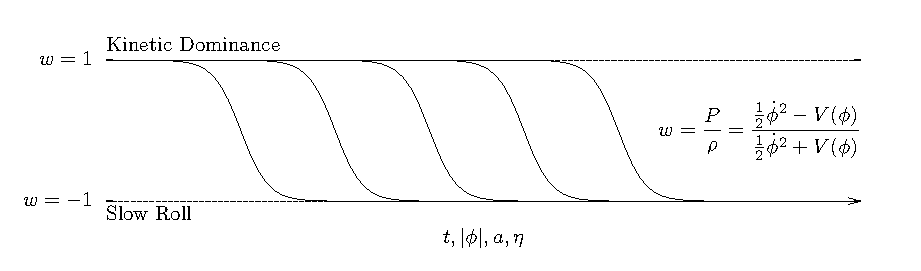
\includegraphics[width=\textwidth]{chapter_kinetic_thoughts/plots/w.tikz}
  \caption{%
    Schematic of the equation of state parameter $w$ against cosmic
    evolution. The generic scenario entails beginning in a kinetically
    dominated phase with $w=1$ (i.e.\ $\dot{\phi}^2\gg V(\phi)$)
    before moving to the typical slow roll attractor solution with
    $w=-1$ (i.e.\ $\dot{\phi}^2 \ll V(\phi)$). We term the
    intermediate stage ``Fast roll''.\label{fig:kt:w}
  }
\end{figure}
%%%%%%%%%%%%%%%%%%%%%%%%%%%%%%%%%%%%%%%%%%%%%%%%%%%%%%%%%%%%%%%%%%%%%%

The statements above are rigorously true. However, the key question is how physically relevant this observation is, and how this relates to more traditional inflationary set-ups and assumptions.

The classical equations have two opportunities to break down. First, it may be that this kinetically dominated state occurs before the Planck time, when we know that we would need a quantum theory of gravity to describe the universe. Second, it may be that the homogeneity assumption breaks down at early times.

\section{The Planck time}
The Planck epoch occurs at the earliest times and is defined as the
regime in which we are certain we would need a quantum theory of
gravity. Effectively this occurs when:
\begin{equation}
  \rho = \frac{1}{2}\dot\phi^2 + V(\phi)  \sim \m^4
  \label{eqn:kt:rhosim}
\end{equation}
If the universe exits the kinetically dominated solutions before the
Planck time, then kinetic dominance cannot be physically relevant. We
may use this to put bounds on $\phip$, or alternatively the total
number of $e$-folds of inflation.

If we are in the kinetically dominated phase with $\dot{\phi}^2\gg
V(\phi)$ then:
\begin{equation}
              \rho \approx \frac{1}{2}\dot\phi^2= \frac{1\m^2}{3t^2} 
  \label{eqn:kt:rhop}
\end{equation}
so $\rho\sim\m^4$ implies that $t\sim\tp=\m^{-1}$. Thus, in order for
kinetic dominance to be true at the Planck time we require that:
\begin{equation}
  V(\phip) \ll \m^4
\end{equation}
For $V(\phi) = \frac{1}{2}m^2\phi^2$ inflation, this amounts to requiring that $m^2\phip^2\ll \m^4$. In order to agree with CMB observations, we require
that $m\sim10^{-5}\m$, which amounts to requiring that:
\begin{equation}
 \phip^2 \ll 10^{10}\m^2 \nonumber.
 \label{eqn:kt:phipbound}
\end{equation}

We may phrase this in terms of the total number of $e$-folds:
\begin{align}
  N_\mathrm{tot} 
  &=\int_{t_\mathrm{begin}}^{t_\mathrm{end}} H dt 
  =\int_{\phi_\mathrm{begin}}^{\phi_\mathrm{end}} 
       \frac{H}{\dot{\phi}}d\phi  &\text{($H=\dot{N}$)}
  \\
  &=\frac{1}{\m^2}\int_{\phi_\mathrm{begin}}^{\phi_\mathrm{end}}
     {\frac{V(\phi)}{V^\prime(\phi)}}d\phi &\text{Slow Roll.}
\end{align}
For $V\sim\phi^n$, this gives:
\begin{equation}
  N = \frac{\Delta (\phi^2) }{n\:\m^2}
\end{equation}
If we take our upper bound (\ref{eqn:kt:phipbound}), and assume that the
end of inflation is somewhere near the base of the potential, we find
that: 
\begin{equation}
  N_\mathrm{tot}\ll 10^{10}.
\end{equation}
It is difficult to imagine how one could possibly constrain the total
number of $e$-folds observationally, unless the number was
sufficiently small so as to be observable directly in the CMB power
spectrum (for example in ``just enough inflation''). There are
theoretical limits, but these typically tend to be much, much larger
than this.

\section{Eternal inflation}
Theorists typically assume an effectively eternal inflationary phase all the way back to the Planck time.  
The typical argument by Linde goes something like this:
\begin{enumerate}
  \item We should set initial conditions at the Planck time, when
    $\rho\sim\m^4$.
  \item There will be some partitioning between kinetic and potential
    energy at this moment.
  \item Given that we know nothing of the physics we should put
    uniform priors the amount of energy in the potential at this
    moment: $V(\phip)\in[0,\m^4]$.
  \item Therefore on average we expect equipartition between kinetic
    and potential energy at the Planck time
\end{enumerate}

From Linde's argument, the kinetically dominated regime is only present
after the Planck time for $V(\phip)$ at the very bottom end of the
prior range.

We can see this graphically in Figure~\ref{fig:kt:linde}. Solutions are plotted so that they are equally spaced in kinetic energy at the Planck time. Whilst graphs similar to the upper half of the figure is typically shown in lectures and textbooks, this is for an artificially high value of $m$. As $m$ is decreased, the phase space look more like the lower half of Figure~\ref{fig:kt:linde}, and the ``Planck circle'' becomes an elongated ellipse. 

If $m$ is set to the more physically reasonable $m\sim10^5\m$, then it becomes slightly less reasonable to suggest that the universe could emerge uniformly within five orders of magnitude. It might be just as reasonable to suspect a logarithmic prior.

Additionally, if one sets the equipartition between kinetic and potential energy after inflation, then a very different picture is painted, as in Figure~\ref{fig:kt:b4infl}. Here almost all solutions begin in a kinetically dominated phase. 

The problem is that all of these arguments tend to the more philosophical end of physics: ``What is the natural prior to assume on initial conditions''. It is far better to try and answer these questions observationally. If the kinetically dominated phase is observable, then all of this is moot.

\begin{figure}[tp]
  \centering
  \tikzsetnextfilename{swirl}
  \includegraphics[width=\textwidth]{chapter_kinetic_thoughts/plots/swirl.tikz}
  \tikzsetnextfilename{true}
  \includegraphics[width=\textwidth]{chapter_kinetic_thoughts/plots/true.tikz}
  \caption{Phase-space plot of the evolution of $(\phi,\dot{\phi})$ for a chaotic inflationary potential $V(\phi) = \frac{1}{2}m^2 \phi^2$. The upper plot has $m=0.5\m$. The outer circle is the Planck time $\tp$ when $\rho=\m^4$. One can see that each path through phase space is generically drawn to the slow roll attractor solutions in the center of the plot. The lines are plotted so that they have a uniform spacing of kinetic energy at the Planck time.
  The upper plot is somewhat misleading, since it has an artificially high value of $m$. When the value of $m$ is lowered to $0.1\m$, as in the lower plot, then the slow roll phase is a much stronger attractor solution, and generates a sustained slow-roll accelerated expansion.\label{fig:kt:linde}}
\end{figure}

\begin{figure}[tp]
  \centering
  \tikzsetnextfilename{swirl_alt}
  \includegraphics[width=\textwidth]{chapter_kinetic_thoughts/plots/swirl_alt.tikz}
  \tikzsetnextfilename{true_alt}
  \includegraphics[width=\textwidth]{chapter_kinetic_thoughts/plots/true_alt.tikz}
  \caption{Phase space plot as in Figure~\protect\ref{fig:kt:linde}, but with initial conditions uniform in kinetic energy after the inflationary phase. The solutions which uniformly distribute their energy after inflation now predominantly begin at the Planck time in a more kinetically dominate state. As one decrease $m$ to more physical values (lower plot) almost all early-time solutions are kinetically dominated.\label{fig:kt:b4infl}}
\end{figure}




\section{Breakdown of homogeneity}
We have shown that all homogeneous universes classically begin in a kinetically dominated phase. It is profitable to examine the form of the perturbed equations~\eqref{eqn:cos:einsteins_equations_perturb}, to take into account the evolution of any spatial variation in the solutions.

To first order, the $i$-$j$, $i$-$0$ and $0$-$0$ Einstein equations read:
\begin{align}
  \Phi &= \Psi 
  \label{eqn:kt:Eij} \\
  0 &= -\dot{\phi}\:\delta\phi  + 2 H \Phi + 2 \dot{\Phi} 
  \label{eqn:kt:Ei0}\\
  0 &= \left(6H^2-\dot{\phi}^2 + 2\frac{k^2}{a^2}\right)\Phi  + \left( -3H\dot{\phi} - \ddot{\phi} \right)\delta\phi + \dot{\phi}\delta\dot{\phi} +  6 H \dot{\Phi},
  \label{eqn:kt:E00}
\end{align}
where we have absorbed the explicit potential dependence into $\ddot{\phi}$ terms. 
One may rearrange these to gain second order equations in $\Phi$ or $\mathcal{R}$:
\begin{align}
  0 &= \ddot{\Phi} + \left( H - 2 \frac{\ddot{\phi}}{\dot{\phi}} \right) \dot{\Phi} + \left( \frac{k^2}{a^2}-\frac{1}{\m^2}\dot{\phi}^2 - 2\frac{\ddot{\phi}}{\dot{\phi}}H \right)\Phi, \\
  0 &= \ddot{\mathcal{R}} + \left( \frac{\dot{\phi}^2}{\m^2H} + 3H + 2\frac{\ddot{\phi}}{\dot{\phi}} \right)\dot{\mathcal{R}} + \frac{k^2}{a^2}\mathcal{R}, \qquad \mathcal{R} = \Psi - \frac{H}{\dot{\phi}}\delta\phi
\end{align}
There is of course also a second order equation purely in $\delta\phi$, but this is particularly unappetising, and given that we have an explicit solution for it in~\eqref{eqn:kt:Ei0}, we shall not state it here.
Technically, these equations are derived in the Newtonian gauge ($E=B=0$), but since everything here is manifestly gauge invariant one may interpret all of the above equations as the relations in the equivalent gauge invariant variables.

If we apply the kinetically dominated solutions to the background variables, we arrive at:
\begin{align}
  0 &= \ddot{\Phi} + \frac{7}{3}\frac{1}{t}\dot{\Phi} + \frac{k^2}{a^2} \Phi,\\
  0 &= \ddot{\mathcal{R}} + \frac{1}{t}\dot{\mathcal{R}} + \frac{k^2}{a^2} \mathcal{R},\\
  a &\propto t^{1/3}
\end{align}
Both equations are solvable with Bessel functions as:
\begin{align}
  0 &=\ddot{x} + (1+p)\frac{1}{t}\dot{x} + \frac{k^2}{a^2} x,  \\
  \Rightarrow \qquad
  x &= t^{-\frac{p}{2}}\left[ A J_{\frac{3}{4}p}\left( \frac{3k}{2a} t \right) + B Y_{\frac{3}{4}p}\left( \frac{3k}{2a} t \right) \right], \\
  &\sim  t^{-\frac{p}{2}-\frac{1}{3}}, \qquad t \gg 1,
\end{align}
where $A$ and $B$ are integration constants. The solutions are generically oscillatory with a polynomial decay with power $-\frac{p}{2} - \frac{1}{3}$.

Physically that means that as we integrate further backwards in time, although the homogeneous universe is drawn toward a kinetically dominated state, spatial inhomogeneities begin to increase.

Thus, if some portion of the universe at an early stage has $\dot{\phi}^2 \gg V(\phi)$, and is approximately homogeneous, then evolving forwards in time the comoving size of that portion will grow, and kinetic dominance causes patches of the universe to homogenise.

Equally, this means that there will be a breakdown in the homogeneity assumption at early times. It remains to be determined at what moment this breakdown occurs for physically observable scales in the early universe. More analytical investigation is required, and is a subject of my current research.

%\cleardoublepage{}
